\chapter{Escaping from transient chaos with partial control} %5P1
\label{chap:ForcingEscape}


\begin{quotation}
	\vspace{-3cm}
    \begin{flushright}
    \begin{minipage}[t][5cm][b]{0.5\textwidth}
    {\letquote ``Fantasy is hardly an escape from reality. It's a way of understanding it."}
    
    \bigskip
    
    -{\small  Lloyd Alexander}
    \end{minipage}
    \end{flushright}
    
    \vspace{0.5cm}
\end{quotation}




Partial control has been developed as a control method generally used in chaotic transients, where the controller does not fix a given orbit, but instead chooses a set of points to avoid. In this chapter we introduce this concept to further develop it in the two following chapters, where we use the partial control method to solve a game between two players. 

The partial control method was firstly introduced to solve the Yorke's Game of Survival in \cite{Yorke'sGame} where a game is defined between a ``protagonist" and an ``antagonist". The goal of the protagonist was to survive in a chaotic transient region indefinitely. In the former paper's case, to keep the orbit in the region $[0,1]$ with the slope three tent map $f(x) = \mu(1-|x|)-1$. The antagonist role was interpreted by the effect of an additive noise, which bound was larger than the control bound of the protagonist.

This map is well known and the iteration of the map in the sequence $x_{i+1} = f(x_i)$ for slopes greater than two, presents transient chaos. This is because the map is only positive for the region $[-1,1]$ and for those slopes, the orbits leave that region after falling near $0.5$ and escape towards $-\infty$. Through the iteration of the map all initial points eventually escape, since only the zero-measure Cantor ternary set remains an indefinite amount of time in the chaotic transient. The escape times depend on the initial conditions and present fractality. Therefore they are highly unpredictable in the disturbed case as can bee seen on Fig.~\ref{fig:EscapeTimes}. Orbits that start near the Cantor set take many iterations to escape without disturbance. Although in Fig.~\ref{fig:EscapeTimes} we used the logistic map, the graphic is similar for the tent map.

Given that all points eventually escape and that the noise bound is greater it is unlikely that the protagonist could survive. However, with the partial control method, it is possible to find sets of points called the safe set for each combination of control bound and noise bound. Given a noise bound and a control bound there is a unique set that enables the protagonist to stay in the region if the initial conditions belongs to the set, for as long as control is active. The sets were firstly found by using the sculpting algorithm \cite{Sculpting} and later the safe functions were developed which enable to find multiple safe sets for different control bounds more efficiently \cite{SafeSets}.

But what drives the study presented in this chapter is not to maintain the orbits in the chaotic region, but to take out the unpredictable manner in which orbits escape from the region. We aim to control the orbits in order of being certain to know how the orbits will escape. We will get some functions similar to the safe functions that allows us either to escape from the chaotic transient region in the least iterations possible, or to set the exact number of iterations that passes before the orbits escape. We called these functions the escape functions, and the sets, the escape sets.
 
\section{Escape from a region with partial control.}

Given a map $f(x)$, with a bounded additive noise $\xi_n$ that affects the map at each iteration $n$, we eject a bounded additive control $u_n$, which, as we mentioned earlier, can be smaller than the noise bound. We define the iterated map that acts on $q\in Q$, $Q$ being a region in phase space as:

\begin{equation}
\begin{split}
&q_{n+1}=f(q_n)+\xi_n+u_n \\
&|\xi_n|\leq \xi_0 \\
&|u_n|\leq u_0.
\end{split}
\end{equation}

The goal is to find the correct sequence of controls ($u_1$, $u_2$,..., $u_m$) to ensure that at the $m^{th}$ iteration, with $m \leq N$, the point $q_{m+1}$ is outside of the region $Q$. $N$ is the maximum number of iterations it will take to achieve the goal, but in some cases, depending on the initial condition, the orbit can be expelled sooner. When setting a very small $N$, the control bound should be high, or otherwise achieving the goal may not be possible. On the other hand, by setting a large $N$ the control bound can be smaller and smaller.

To apply this control technique one should firstly choose the region $Q$ from where the orbits must escape. Then one should compute $N$ quick escape functions $U_k$, $k = 1:N$, which depend on the value $\xi_0$. This functions tell how much control is needed to expel the orbit in $k$ iterations or less.

Then, by setting the control bound $u_0$ compute the escape sets $E_k$ for every escape function. Every point which belongs to this set can be thrown out from the region $Q$ in $k$ or fewer iterations. Each escape set contains all the points which have a value of $U_k$ lower than $u_0$. Since $E_N$ may not gather every point in the region $Q$, if the orbit starts in one of those point that are not gathered in $E_N$, the escape is not guaranteed to be made in $N$ iterations, and could take larger times.

Now, when all escape sets are computed, the control strategy is to push the point $f(q_i) + \xi_i$ towards the escape set with the lower index $k$ that is within control reach.

We also developed a similar algorithm to make the escape from the region $Q$ in an orderly manner, i.e., to escape in exactly $N$ iterations, no more, no less. The procedure is the same as we have explained above, except that the escape functions are different and for the control strategy we have to push the first point towards $E_N$, the second iteration towards $E_{N-1}$ and so on, until the controlled orbit gets to $E_1$ after which the application of the map, noise, and control, the point is outside region $Q$.

Finally we presented a practical case in which we shift the trajectory from one chaotic region to another periodically, resulting in a quasiperiodic orbit.

\section{Application of the method}

%TODO trajectorias 

To give an example on how to apply the algorithms, we have chosen the logistic function $f(x) = \mu x(1-x)$. For $\mu > 4$ there is a chaotic transient on the region $Q=[0,1]$. 

\begin{figure}
    \centering
    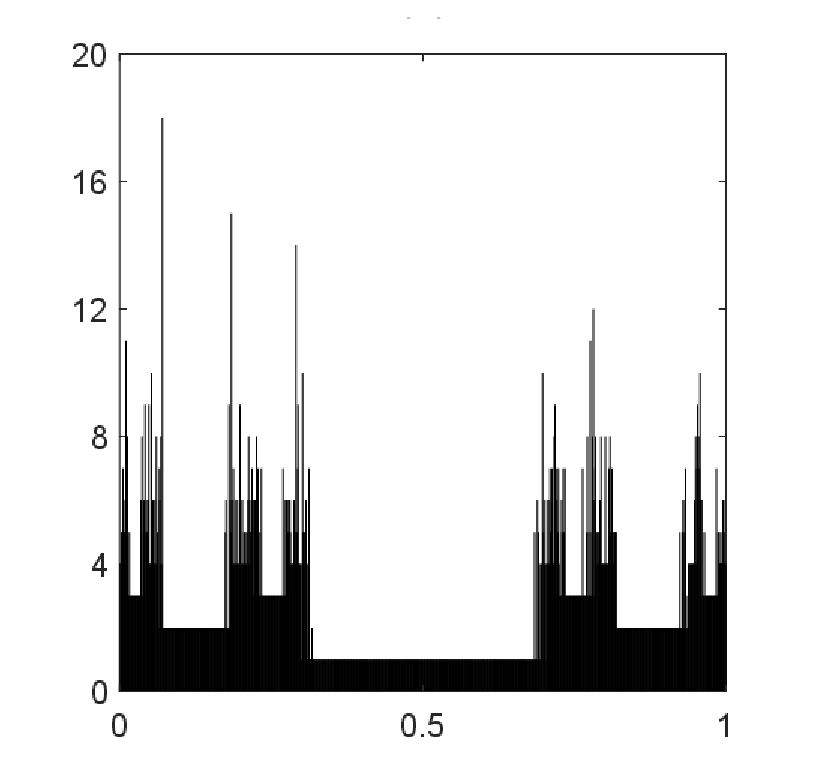
\includegraphics[width=0.5\linewidth]{Images/P1/EscapeTimes.eps}
    \caption{Escape times from the chaotic transient of the logistic map with $\mu=4.7$ and a noisy disturbance bounded to $\xi_0 = 0.03$. Horizontal axis represents the starting points for the orbit and the vertical axis, the number of iterations of a random orbit before it escaped the chaotic transient region $Q = [0,1]$}
    \label{fig:EscapeTimes}
\end{figure}

In the following subsections we present the algorithms to calculate the escape functions and sets in order to achieve three distinct goals. First, to make the orbits escape region $Q$ as quickly as possible setting a maximum number of iterations $N$. Next, to set an exact number of iterations $N$ after which the orbit must be outside region $Q$. Finally, to make a quasiperiodic orbit that shifts between two chaotic transients at fixed intervals $N_1$ and $N_2$ iterations. 

\subsection{Escaping as quick as possible}

We want to make orbits to escape in $N$ iterations or less. The larger the control bound is, the quicker some orbits will escape and the escape sets will be broader. This will be helpful if one wishes to avoid as much as possible chaotic orbits which can be dangerous in some situations. The authors of \cite{AvoidTransient1} state that ``transient chaos may be a dangerous and unwanted state of a vibro-impact system". 

Since we are making numerical calculations, we must use a grid on region $Q$. We divide the region in $M$ equal parts, so that the region transforms in a collection of equidistant points $q[i]$, $i=1:M$. Also the value of the noise is discretized into $W$ values ranging from $-\xi_0$ to $\xi_0$. The map then becomes:

\begin{equation}
    q[j] = f(q[i]) +\xi[s] +u[i,s,j],
\end{equation}
where $q[j]$ is the arrival point with $j=1:M$. Now we are ready to compute the escape functions.

Firstly we compute the escape function $U_1$. This function tells us the control necessary for every point in the region $Q$ to escape in the next iteration. 
\begin{equation}
U_1(q[i]) = \max\limits_{s}(min(f(q[i]) + \xi[s] + \epsilon - 0, 1 + \epsilon - (f(q[i]) + \xi[s]))),
\end{equation}
where $0$ and $1$ are the limits of the region $Q$ and $\epsilon$ is a small number to ensure the escape and is convenient to be $1/M$.

If $f(q[i]) + \xi[s]$ is beyond $Q$ then change the function value to $0$, since there is no need for control.

Then, we calculate the following functions recursively with this formula:

\begin{equation*}
u[i,s,j] = q[j] - f(q[i]) - \xi[s]
\end{equation*}
\begin{equation*}
U^{*}_{k+1}[i]=\max_s\Big(\min_j\big(\max(|u[i,s,j]|,U_k[j])\big)\Big)
\end{equation*}
\begin{equation}
U_{k+1}[i]=\min\bigg(U_k[i],U^{*}_{k+1}[i]\bigg),
\label{equ:QuickEscapeFunctions}
\end{equation}
where $u[i,s,j]$ is the control to take the resulting point, after the application of the map and noise, to each point in the grid. The last equation ensures that the escape can be done in less than $N$ iterations.

\begin{figure}
    \centering
    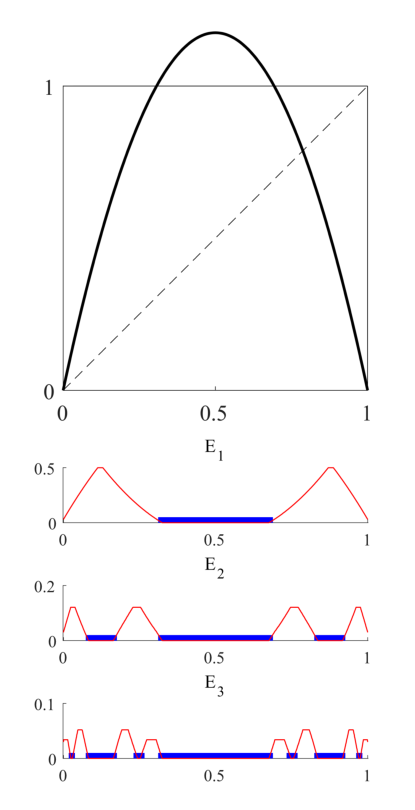
\includegraphics[width=0.4\textheight]{Images/P1/EscapeSetsQuick.eps}
    \caption{On top, logistic map $\mu x(1-x)$ with $\mu = 4.7$. On the bottom, escape functions (red) and escape sets (blue) for escaping in $N=3$ or less iterations as quick as possible. The functions were computed for a noise bound of $\xi_0 = 0.03$ and the sets for a control bound of $u_0 = 0.022$. The vertical axis shows the minimum control needed for orbits starting at each starting point to stay in the chaotic transient region $Q = [0,1]$ indefinitely, which mark the quick escape functions in red. The quick escape sets $E_k$ are highlighted in blue and their heights are trivial. The points in these sets can be controlled with the given control bound to escape in at maximum $i$ iterations.   }
    \label{fig:EscapeSetsQuick}
\end{figure}

We give an example with $N=3$ in Fig.~\ref{fig:EscapeSetsQuick}. The escape sets in blue are the regions of the escape functions in red that have lower value than the control bound. Each index $k$ in $E_k$ tells in how many iterations is possible to escape. 

Now in order to escape as quick as possible one needs to push the iterated point of the orbit towards the lowest indexed escape set reachable. 

By increasing the number of iterations we allow for the orbit to escape $N$, the escape sets will become larger. For $N\to\infty$ the set becomes the entire region except the zero-measure Cantor ternary set. This will not be the case for the following case in which the orbit must escape at an exact number of iterations.


\subsection{Escaping at an exact number of iterations}

Now we ask ourselves if it is possible to set the exact number of iterations before an orbit is expelled from the chaotic transient. This seems a difficult task when considered the restriction of limiting control to be smaller than noise, since some points naturally escape in one iteration, while others take a lot of time to do so. 

However, we repeat the same line of work as the previous case, by constructing the exact escape functions and later by getting the exact escape sets. When inspecting the logistic map, points at the center will escape naturally in the next iteration, so probably these points won't be in the exact escape sets for large values of their index. On the other hand points near the Cantor ternary set seem to be out of bounds for the sets with small index. This landscape will be reflected on the exact escape functions which are constructed differently than in the previous case.

In spite of the task seeming harder, the algorithm to calculate the escape functions is very similar and even simpler. $U_1$ is calculated the same obviously. Then the rest of the functions are computed exactly as equations~\ref{equ:QuickEscapeFunctions} but without the last equation. In this case, we do not check whether the function is smaller than the function with lower index since we cannot allow for an earlier escape.

\begin{equation*}
u[i,s,j] = q[j] - f(q[i]) - \xi[s]
\end{equation*}
\begin{equation}
U_{k+1}[i]=\max_s\Big(\min_j\big(\max(|u[i,s,j]|,U_k[j])\big)\Big)
\label{equ:ExactEscapeFunctions}
\end{equation}





\begin{figure}
    \centering
    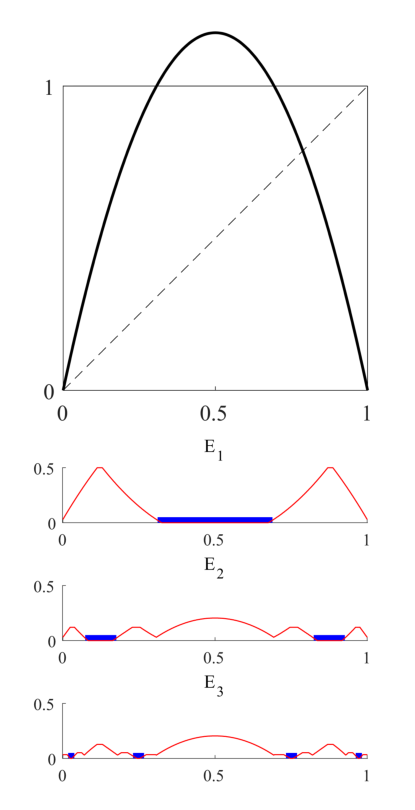
\includegraphics[width=0.4\textheight]{Images/P1/EscapeSetsExact.eps}
    \caption{On top, logistic map $\mu x(1-x)$ with $\mu = 4.7$. On the bottom, escape functions (red) and escape sets (blue) for escaping in $N=3$ or less iterations as quick as possible. The functions were computed for a noise bound of $\xi_0 = 0.03$ and the sets for a control bound of $u_0 = 0.022$. The vertical axis shows the minimum control needed for orbits starting at each starting point to stay in the chaotic transient region $Q = [0,1]$ indefinitely. The blue lines mark the exact escape heights $E_k$, their heights are meaningless, the points highlighted can escape in exactly $k$ iterations with the given control bound. }
    \label{fig:EscapeSetsExact}
\end{figure}




Following this formula, we arrive to the exact escape functions and sets in Fig.~\ref{fig:EscapeSetsExact}. We can see that the sets are smaller, because the set $E_k$ doesn't contain the contents of $E_{k-1}$, unlike the previous case. Each exact escape set $E_k$ is the complementary of the $k-th$ approximate Cantor ternary set $C_k$, though a little bit decreased or increased depending on whether the noise is greater than the control or vice versa. 

Now, to escape in exactly $N$ iterations, we must simply take the first iterated point towards $E_{N-1}$. This will be possible only if the initial point started in $E_N$. Afterwards we will push the iterated point one escape set further at a time until $E_1$ is reached. Then, after iterating the map the orbit will be out of the chaotic region or the border will be within reach.




\subsection{Shifting chaotic transients}
 

Thanks to the previous control method we can accurately control the escape from a chaotic transient in an orderly manner. This can be helpful in a case where a rigorous control of time is needed. This next case goes forward in this direction, by setting the frequencies of time at which a controlled orbit shifts from one chaotic transient to another. With this control technique one can build a chaotic clock in which a desired chaotic system changes significantly at some desired rates and still maintaining its chaotic behavior. 

This can be useful in multistable chaotic systems. In these kind of systems, varying a parameter one can merge various atractors into a larger one with different regions when their basin boundary collides. The orbit shifts chaotically from one region to the other continuously \cite{Multistable2}. One example of this motion is the Lorentz system \cite{Lorentz}, and others are given in \cite{Multistable2, Multistable3, Multistable4}.

With the following control method, one could make this shifts to appear periodically as long as control is made while maintaining the chaotic motion through the rest of the orbit. The orbit will therefore be quasi-periodical.

We will develop this method on a simple model to show the procedure. On the top graphic of Fig.~\ref{fig:ShiftSets} we show the custom made double parabola map:

\begin{equation}
f(x) = \left\{ \begin{array}{ll}
-\mu (x^2 - \dfrac{1}{2}x)  & \mbox{if $x<0.5$,} \\
1 + \mu (x^2 -\dfrac{3}{2}x + \dfrac{1}{2})  & \mbox{if $x\geq 0.5$,} 
\end{array}
\right.
\end{equation}

The bifurcation diagram and Lyapunov exponent for the iterated map $x_{n+1} = f(x_n)$ are shown in Figures \ref{fig:Bifurcation} and \ref{fig:Lya} respectively. It shows that there is a chaotic behavior for most values of $mu > $ and for values of $ < \mu < 8$ there are two separated atractors that merge at $\mu = 8$ into a larger one. Then, for values close to that, the orbit shifts chaotically between the left and right regions. 

Figure~\ref{fig:TrajectoryDouble} shows this shifts in the uncontrolled trajectory at the top and how we have controlled them, resulting in a quasi-periodic orbit with periodic shifts between the two regions. Also, we can see how the magnitude of the control made at each iteration is lower than the noise bound.


\begin{figure}
    \centering
    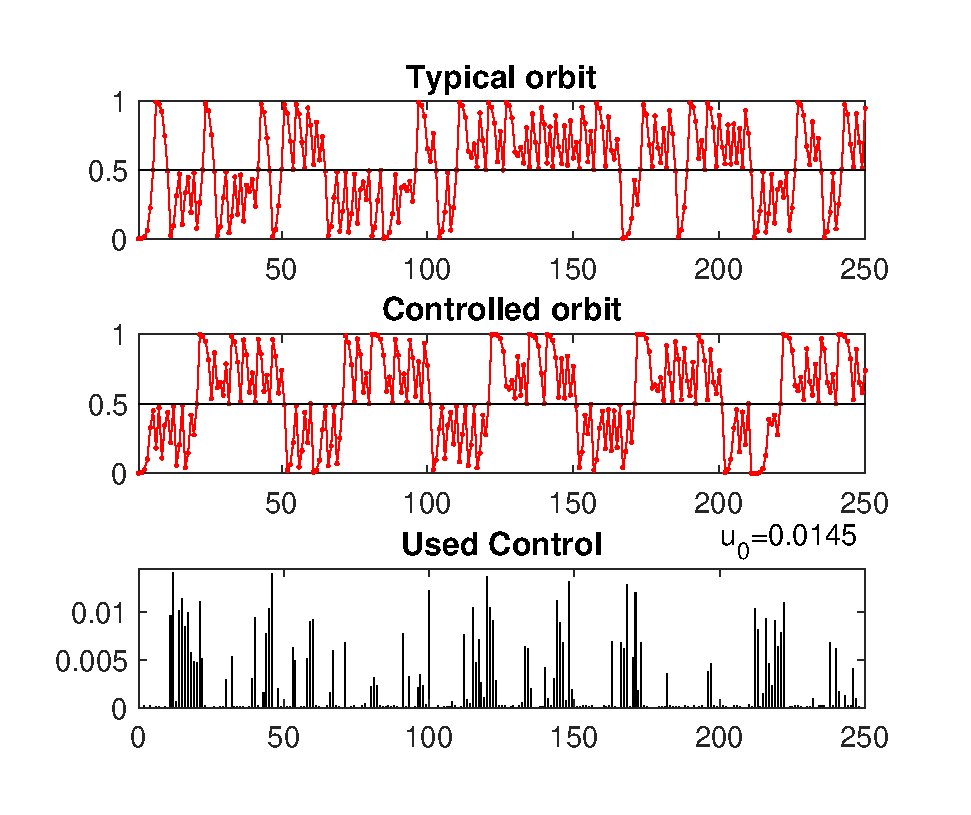
\includegraphics[width=0.7\textheight]{Images/P1/Alt_tray_mu8.1.eps}
    \caption{Controlled and uncontrolled orbits of the double parabola map for $\mu = 8.1$ in red. The typical orbit describes the motion of a chaotic system where the attractor has different regions. The orbits stay an indefinite amount on each side of the attractor shifting chaotically. This is typical of a multistable chaotic system in the moment when its different attractors have merged into a larger one. We were able to control the dynamics in the map so it keeps the chaotic behavior in each side of the attractor, but have controlled the frequency of the shifts. As we can see the controlled orbits spends $N^l = 20$ iterations at the left side and $N^r = 30$ at the right one. The control made at each iteration was at most the value of its bound $u_0 = 0.0145$ which is lower than the noise bound $\xi_0 = 0.015$}
    \label{fig:TrajectoryDouble}
\end{figure}



This control has been calculated following the same approach as the previous cases. In this case through the shift functions and sets. These are similar than the escape sets and are calculated taking into account the control $u_{in}^l$ as the control needed to get an iterated point in region $Q^l$ to another desired point in the same region, calculated as:
\begin{equation*}
u_{in}^{l,r}[i,s,j] =  q^{l,r}[j] - f(q^{l,r}[i]) - \xi[s].
\end{equation*}

Also important is the control $u_{out}^{l,r}$ needed to get one point from region $Q^{l,r}$ to the opposite region $Q^{r,l}$. This is:
\begin{equation*}
u_{out}^{l,r}[i,s,j] = q^{r,l}[j] - f(q^{l,r}[i]) - \xi[s].
\end{equation*}



\begin{algorithm}[h!]
    \caption{\textbf{Iterative process to calculate the shift functions $U^{l,r}_{k}$ to stay in the left or right side of the double parabola map a number of iterations $N^l$ and $N^r$ respectively.} }
    \label{alg:ShiftFunction}
\renewcommand{\thealgorithm}{}
\floatname{algorithm}{}

\begin{algorithmic}[0]
    \While{$U^{l,r}_{k}$ \text{are different than previous iteration}} 
    
        \For{$k=1:N^l-1$}

          \State  $U^{l}_{k+1}(q[i])=\max\limits_s\Big(\min\limits_j\big(\max(u_{in}^l[i,s,j],U^l_k(q[j]))\big)\Big)$

        \EndFor
    
       \State   $U^{r}_{1}(q[i])=\max\limits_s\Big(\min\limits_j\big(\max(u_{out}^r[i,s,j],U^l_{N^l}(q[j]))\big)\Big)$   
        
        \For{$k=1:N^r-1$}
        
            \State  $U^{r}_{k+1}(q[i])=\max\limits_s\Big(\min\limits_j\big(\max(u_{in}^r[i,s,j],U^r_kq([j]))\big)\Big)$
            
        \EndFor
        
        \State  $U^{l}_{1}(q[i])=\max\limits_s\Big(\min\limits_j\big(\max(u_{out}^l[i,s,j],U^r_{N^r}q([j]))\big)\Big)$
    \EndWhile
    \end{algorithmic}
\end{algorithm}



\begin{figure}
    \centering
    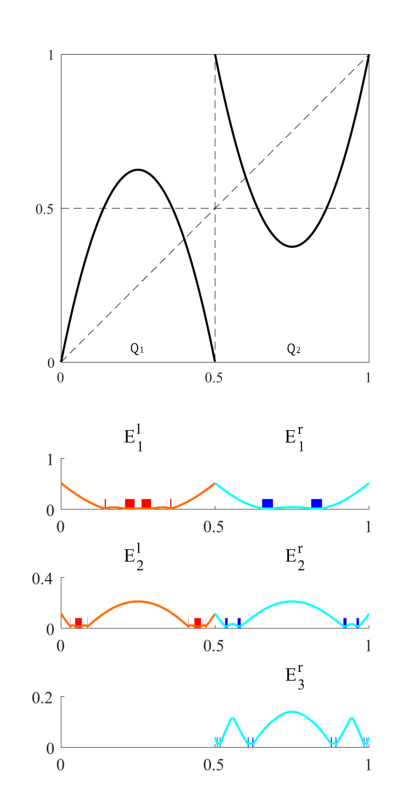
\includegraphics[width=0.4\textheight]{Images/P1/Alt_sets.eps}
    \caption{On top, the custom made double parabola map for $\mu = 10$. It present two differentiated zones at left and right of the middle point at $0.5$. At the bottom we present the shift functions as lines and sets as blocks. The shift fucntions $U^{l,r}_k$ tells how much control is needed at least to keep the orbit in the left or right region for $k$ iterations before shifting to the other region. In this case we have calculated the functions and sets in order to keep the orbit $N^l = 2$ iterations at the left and $N^r = 3$ iterations to the right.}
    \label{fig:ShiftSets}
\end{figure}





Taking as a seed $U^l_1 = 0$,  we can calculate the shift functions $U^{l,r}_k$ following Algorithm~\ref{alg:ShiftFunction}, which tell the control needed to be able to control the orbit $k$ iterations at the left or right region before shifting to the other region.  The shift sets $E^{l,r}_k$ will be the set of points that has a lower value of the function than their bound of control. They are ordered like the exact escape sets from previous section, the upper letter indicating if the escape set is from the left or right region $Q^{l,r}$, and their index $k$ indicating the number of iterations needed until the orbit will shift to the other region. 

An example is given in Fig.~\ref{fig:ShiftSets}. We calculated the shift sets in order for the orbit to remain $N^l = 3$ at the left side, and $N^r = 2$ at the right side. Following the example, if an orbit starts at a point in $E^l_3$ it will arrive at $E^l_2$ and then $E^l_1$ through control after which, it can be controlled to shift to $E^r_2$, then repeating the same process on the right side until the orbit can be shifted to the left. This process can be continued indefinitely. If one is fortunate and the orbit starts at a point with low value of the shift function, the control can be made lower than the noise.


\section{Conclusions}

We have applied the partial control method with the goal of driving off trajectories from a chaotic transient region. We developed two methods of doing this. Firstly the controller may want to expel the trajectory as swift as possible. Alternatively, the control can be made in an orderly manner, choosing the exact number of iterations that the trajectory stays at the transient region from the beginning of control to the moment the trajectory leaves the region.

Another case was studied in which the controller shifts periodically between two regions of a multistable chaotic system. In these kind of systems the trajectory shift in chaotic manner from one region to the other, but with the control method provided here, we controlled the frequency of these shifts. The result is a quasi-periodic orbit in which there is a periodical shifting through the two regions, but the orbit inside each region remains chaotic.

The control method does not provide a given orbit to follow strictly, but instead analyses the system and finds sets of points reachable within control limits that serve to complete the goal. The controller can then choose from those points, whether randomly or with other priorities in mind, where to direct the orbit. The outstanding fact about this control method is that there are occasions in which the maximum control can be set to be lesser than a known noise bound.

A simple example is given for each of the three cases. The logistic map was studied in the first two cases and for the control of a multistable system, we crafted a custom made map consisting of two disjointed parabolas with opposite convexity.

For all the cases we managed to achieve the goal at some set of initial conditions even when control was lesser than noise. Increasing the control ensures that more initial conditions are able to be controlled.






















\clearpage



\begin{thebibliography}{05}

\bibitem{Yorke'sGame}
J. Aguirre, F. d’Ovidio, and M. A. F. Sanjua´n
Controlling chaotic transients: Yorke’s game of survival
Phys. Rev. E 69:016203 
(2004)


\bibitem{Sculpting}
J. Sabuco, S. Zambrano, M. A.F. Sanjuán, and J. A. Yorke,
Finding safety in partially controllable chaotic systems.
Commun Nonlinear Sci Numer Simulat 17:4274–4280 
(2012)


\bibitem{SafeSets}
R. Capeáns, J. Sabuco, M. A. F. Sanjuán
A new approach of the partial control method in chaotic
systems.
Nonlinear Dyn 98:873–887 
(2019) 


\bibitem{AvoidTransient1}
V.A. Bazhenov, O. S. Pogorelova, and T.G. Postnikova,
Transient chaos in platform-vibrator with shock.
Strength Mater. Theory Struct. \textbf{106} 22-40 
(2021)


\bibitem{Multistable1}
Y.~F. Jin,
{\em Stochastic resonance in an under-damped bistable system driven by harmonic mixing signal}, 
Chinese Phys B \textbf{27}, 050501 
(2018)


\bibitem{Lorentz}
E. N. Lorenz,
Deterministic nonperiodic flow.
J. Atmos. Sci. \textbf{20}:130-141 
(1963)



\bibitem{Multistable2}
E.~L. Rempel and A.~C.-L. Chian, 
{\em Intermittency induced by attractor-merging crisis in the kuramoto-sivashinsky equation}, 
Phys Rev E \textbf{71}, 016203 
(2005)

\bibitem{Multistable3}
A.~L. Livorati, I.~L. Caldas, C.~P. Dettmann, and E.~D. Leonel,
{\em Crises in a dissipative bouncing ball model},
Phys Lett A \textbf{379}, 2830--2838 
(2015)

\bibitem{Multistable4}
S.~Vaidyanathan, S.~T. Kingni, A.~Sambas, M.~A. Mohamed, and M.~Mamat,
{\em A new chaotic jerk system with three nonlinearities and synchronization via adaptive backstepping control},
Int. J. Eng. Technol. \textbf{7}, 1936--1943 
(2018)




\end{thebibliography}